\documentclass[a4paper,11pt,oneside]{memoir}

% Castellano
\usepackage[spanish,es-tabla]{babel}
\selectlanguage{spanish}
\usepackage[utf8]{inputenc}
\usepackage{placeins}

\RequirePackage{booktabs}
\RequirePackage[table]{xcolor}
\RequirePackage{xtab}
\RequirePackage{multirow}

% Links
\usepackage[colorlinks]{hyperref}
\hypersetup{
	allcolors = {red}
}

% Ecuaciones
\usepackage{amsmath}

% Rutas de fichero / paquete
\newcommand{\ruta}[1]{{\sffamily #1}}

% Párrafos
\nonzeroparskip


% Imagenes
\usepackage{graphicx}
\newcommand{\imagen}[2]{
	\begin{figure}[!h]
		\centering
		\includegraphics[width=0.9\textwidth]{#1}
		\caption{#2}\label{fig:#1}
	\end{figure}
	\FloatBarrier
}

\newcommand{\imagenflotante}[2]{
	\begin{figure}%[!h]
		\centering
		\includegraphics[width=0.9\textwidth]{#1}
		\caption{#2}\label{fig:#1}
	\end{figure}
}



% El comando \figura nos permite insertar figuras comodamente, y utilizando
% siempre el mismo formato. Los parametros son:
% 1 -> Porcentaje del ancho de página que ocupará la figura (de 0 a 1)
% 2 --> Fichero de la imagen
% 3 --> Texto a pie de imagen
% 4 --> Etiqueta (label) para referencias
% 5 --> Opciones que queramos pasarle al \includegraphics
% 6 --> Opciones de posicionamiento a pasarle a \begin{figure}
\newcommand{\figuraConPosicion}[6]{%
  \setlength{\anchoFloat}{#1\textwidth}%
  \addtolength{\anchoFloat}{-4\fboxsep}%
  \setlength{\anchoFigura}{\anchoFloat}%
  \begin{figure}[#6]
    \begin{center}%
      \Ovalbox{%
        \begin{minipage}{\anchoFloat}%
          \begin{center}%
            \includegraphics[width=\anchoFigura,#5]{#2}%
            \caption{#3}%
            \label{#4}%
          \end{center}%
        \end{minipage}
      }%
    \end{center}%
  \end{figure}%
}

%
% Comando para incluir imágenes en formato apaisado (sin marco).
\newcommand{\figuraApaisadaSinMarco}[5]{%
  \begin{figure}%
    \begin{center}%
    \includegraphics[angle=90,height=#1\textheight,#5]{#2}%
    \caption{#3}%
    \label{#4}%
    \end{center}%
  \end{figure}%
}
% Para las tablas
\newcommand{\otoprule}{\midrule [\heavyrulewidth]}
%
% Nuevo comando para tablas pequeñas (menos de una página).
\newcommand{\tablaSmall}[5]{%
 \begin{table}
  \begin{center}
   \rowcolors {2}{gray!35}{}
   \begin{tabular}{#2}
    \toprule
    #4
    \otoprule
    #5
    \bottomrule
   \end{tabular}
   \caption{#1}
   \label{tabla:#3}
  \end{center}
 \end{table}
}

%
% Nuevo comando para tablas pequeñas (menos de una página).
\newcommand{\tablaSmallSinColores}[5]{%
 \begin{table}[H]
  \begin{center}
   \begin{tabular}{#2}
    \toprule
    #4
    \otoprule
    #5
    \bottomrule
   \end{tabular}
   \caption{#1}
   \label{tabla:#3}
  \end{center}
 \end{table}
}

\newcommand{\tablaApaisadaSmall}[5]{%
\begin{landscape}
  \begin{table}
   \begin{center}
    \rowcolors {2}{gray!35}{}
    \begin{tabular}{#2}
     \toprule
     #4
     \otoprule
     #5
     \bottomrule
    \end{tabular}
    \caption{#1}
    \label{tabla:#3}
   \end{center}
  \end{table}
\end{landscape}
}

%
% Nuevo comando para tablas grandes con cabecera y filas alternas coloreadas en gris.
\newcommand{\tabla}[6]{%
  \begin{center}
    \tablefirsthead{
      \toprule
      #5
      \otoprule
    }
    \tablehead{
      \multicolumn{#3}{l}{\small\sl continúa desde la página anterior}\\
      \toprule
      #5
      \otoprule
    }
    \tabletail{
      \hline
      \multicolumn{#3}{r}{\small\sl continúa en la página siguiente}\\
    }
    \tablelasttail{
      \hline
    }
    \bottomcaption{#1}
    \rowcolors {2}{gray!35}{}
    \begin{xtabular}{#2}
      #6
      \bottomrule
    \end{xtabular}
    \label{tabla:#4}
  \end{center}
}

%
% Nuevo comando para tablas grandes con cabecera.
\newcommand{\tablaSinColores}[6]{%
  \begin{center}
    \tablefirsthead{
      \toprule
      #5
      \otoprule
    }
    \tablehead{
      \multicolumn{#3}{l}{\small\sl continúa desde la página anterior}\\
      \toprule
      #5
      \otoprule
    }
    \tabletail{
      \hline
      \multicolumn{#3}{r}{\small\sl continúa en la página siguiente}\\
    }
    \tablelasttail{
      \hline
    }
    \bottomcaption{#1}
    \begin{xtabular}{#2}
      #6
      \bottomrule
    \end{xtabular}
    \label{tabla:#4}
  \end{center}
}

%
% Nuevo comando para tablas grandes sin cabecera.
\newcommand{\tablaSinCabecera}[5]{%
  \begin{center}
    \tablefirsthead{
      \toprule
    }
    \tablehead{
      \multicolumn{#3}{l}{\small\sl continúa desde la página anterior}\\
      \hline
    }
    \tabletail{
      \hline
      \multicolumn{#3}{r}{\small\sl continúa en la página siguiente}\\
    }
    \tablelasttail{
      \hline
    }
    \bottomcaption{#1}
  \begin{xtabular}{#2}
    #5
   \bottomrule
  \end{xtabular}
  \label{tabla:#4}
  \end{center}
}



\definecolor{cgoLight}{HTML}{EEEEEE}
\definecolor{cgoExtralight}{HTML}{FFFFFF}

%
% Nuevo comando para tablas grandes sin cabecera.
\newcommand{\tablaSinCabeceraConBandas}[5]{%
  \begin{center}
    \tablefirsthead{
      \toprule
    }
    \tablehead{
      \multicolumn{#3}{l}{\small\sl continúa desde la página anterior}\\
      \hline
    }
    \tabletail{
      \hline
      \multicolumn{#3}{r}{\small\sl continúa en la página siguiente}\\
    }
    \tablelasttail{
      \hline
    }
    \bottomcaption{#1}
    \rowcolors[]{1}{cgoExtralight}{cgoLight}

  \begin{xtabular}{#2}
    #5
   \bottomrule
  \end{xtabular}
  \label{tabla:#4}
  \end{center}
}




\graphicspath{ {./img/} }

% Capítulos
\chapterstyle{bianchi}
\newcommand{\capitulo}[2]{
	\setcounter{chapter}{#1}
	\setcounter{section}{0}
	\chapter*{#2}
	\addcontentsline{toc}{chapter}{#2}
	\markboth{#2}{#2}
}

% Apéndices
\renewcommand{\appendixname}{Apéndice}
\renewcommand*\cftappendixname{\appendixname}

\newcommand{\apendice}[1]{
	%\renewcommand{\thechapter}{A}
	\chapter{#1}
}

\renewcommand*\cftappendixname{\appendixname\ }

% Formato de portada
\makeatletter
\usepackage{xcolor}
\newcommand{\tutor}[1]{\def\@tutor{#1}}
\newcommand{\course}[1]{\def\@course{#1}}
\definecolor{cpardoBox}{HTML}{E6E6FF}
\def\maketitle{
  \null
  \thispagestyle{empty}
  % Cabecera ----------------
\noindent
\includegraphics[width=\textwidth]{cabecera}\vspace{1cm}%
  \vfill
  % Título proyecto y escudo informática ----------------
  \colorbox{cpardoBox}{%
    \begin{minipage}{.8\textwidth}
      \vspace{.5cm}\Large
      \begin{center}
      \textbf{TFG del Grado en Ingeniería Informática}\vspace{.6cm}\\
      \textbf{\LARGE\@title{}}
      \end{center}
      \vspace{.2cm}
    \end{minipage}

  }%
  \hfill\begin{minipage}{.20\textwidth}
    
\includegraphics[width=\textwidth]{escudoInfor}
  \end{minipage}
  \vfill
  % Datos de alumno, curso y tutores ------------------
  \begin{center}%
  {%
    \noindent\LARGE
    Presentado por \@author{}\\ 
    en Universidad de Burgos --- \@date{}\\
    \begin{tabbing}
    Tutores: \= Dr. José Francisco Díez Pastor \kill    Tutores: \= Dr. José Francisco Díez Pastor \\    \> Dr. César Ignacio García Osorio    \end{tabbing}
  }%
  \end{center}%
  \null
  \cleardoublepage
  }
\makeatother


% Datos de portada
\title{«Creación de un videojuego y un bot inteligente para el mismo» \\Documentación Técnica}
\author{Pablo Alejos Salamanca}
\tutor{nombre tutor}
\date{\today}

\begin{document}

\maketitle



\cleardoublepage



%%%%%%%%%%%%%%%%%%%%%%%%%%%%%%%%%%%%%%%%%%%%%%%%%%%%%%%%%%%%%%%%%%%%%%%%%%%%%%%%%%%%%%%%



\frontmatter


\clearpage

% Indices
\tableofcontents

\clearpage

\listoffigures

\clearpage

\listoftables

\clearpage

\mainmatter

\appendix

\apendice{Planificación}

\section{Introducción}
A lo largo de este proyecto se ha seguido una metodología ágil


\section{Planificación temporal}

\section{Estudio de viabilidad}

\subsection{Viabilidad económica}

\subsection{Viabilidad legal}



\apendice{Especificación de Requisitos}

\section{Introducción}
En este apartado se especificarán las necesidades funcionales que se pretende alcanzar. Para ello se describirán los requisitos del software que se quiere desarrollar.

\section{Objetivos generales}
\begin{itemize}
    \item Como ya de describió en la memoria, el objetivo del proyecto es diseñar y desarrollar un videojuego de tipo «arcade». Para la implementación del juego que sirve como base para este proyecto, es necesario planear las mecánicas de juego, además de diseñar los modelos del jugador, los enemigos y otros elementos gráficos. Esta tarea también incluye el diseño de la interfaz, banda sonora y efectos de sonido. 
    
    \item Diseñar e implementar un sistema inteligente que posteriormente será utilizado para interactuar con el videojuego creado. Este proceso de divide en:
    \begin{itemize}
        \item Establecer una comunicación entre el juego y el modelo del sistema inteligente. Dado que el juego y el script que hace uso del modelo serán implementados en diferente lenguaje de programación, se debe establecer un mecanismo de intercambio de datos para la comunicación.
        \item Diseñar el conjunto de datos que posteriormente servirá para el entrenamiento del modelo. Al ser el punto de partida el aprendizaje por imitación, necesitaremos un gran volumen de datos de los cuales seleccionaremos todos o solo los más representativos para el entrenamiento.
        \item Implementar, haciendo uso de las bibliotecas como scikit-learn (minería de datos), DEAP(algoritmos evolutivos) y Pandas y NumPy (procesamiento de datos a bajo nivel) el sistema inteligente que jugará al videojuego.
    \end{itemize}
\end{itemize}

\section{Catalogo de requisitos}

\subsection{Especificación de requisitos}
A continuación se procede a describir los requisitos \emph{iniciales} del proyecto. Hay que recalcar que a lo largo del desarrollo se fueron descubriendo carencias que tenían que cubrir nuevas nececidades. Estos nuevos requisitos funcionales no se describen en este apartado, pero pueden ser consultados el la memoria, en el apartado de «Aspectos relevantes».

\subsection{Requisitos funcionales}

\begin{itemize}
    \item RF-1: El juego debe ser de tipo arcade en 2D. Un juego infinito en el que el jugador aspira a alcanzar la máxima puntuación de forma individual. 
    \item RF-2: Controlamos una nave espacial.
        \begin{itemize}
            \item RF-2.1: El jugador tiene una única vida.
            \item RF-2.2: El movimiento del jugador es horizontal.
            \item RF-2.3: El jugador se mueve a velocidad constante.
            \item RF-2.4: El jugador siempre dispara hacia delante en línea recta.
        \end{itemize}
    \item RF-3: El jugador ha de eliminar el máximo número de enemigos posibles sin impactar contra ellos
    \item RF-4: Dos tipos de enemigos
        \begin{itemize}
            \item Tipo básico: 2 vidas
            \item Tipo jefe: 4 vidas
        \end{itemize}
    \item RF-5: Los enemigos aparecen en oleadas y se limitan a avanzar oscilando hacia su objetivo.
    \item RF-6: Cuanto menos se acerquen a la zona inferior de la pantalla mayor será la puntuación que otorgue su eliminación.
    \item RF-7: Si los enemigos llegan a nuestro territorio restarán una cantidad fija de puntos, por lo que nuestra puntuación final se verá notablemente mermada.
    \item RF-8: El juego comienza con la pantalla vacía y el jugador en la parte inferior.
    \item RF-9: Se suma puntos al eliminar enemigos.
    \item RF-10: Cada $0,25$ segundos se debe guardar el estado en forma de instancia en un fichero.
        \begin{itemize}
            \item RF-10.1: La instancia debe tener como mínimo la información de la posicióbn del jugador y la posición de cuatro enemigos. 
        \end{itemize}
\end{itemize}
\apendice{Especificación de diseño}

\section{Introducción}

\section{Diseño de datos}

\section{Diseño procedimental}
A continuación, se procede a explicar algunas nociones relevantes de cómo interactúan entre sí los diferentes elementos que conforman el proyecto. Dado que no es una aplicación al uso, sino que se compone de múltiples elementos, mostraré un diagrama de despliegue y un diagrama de secuencias.

\subsection{Diagrama de despliegue}
La estructura que ha acabado adoptando el proyecto puede resultar algo compleja, por lo que explicaré, en primer lugar, cómo está organizado.

Para empezar es muy importante aclarar que hay dos implementaciones del juego. Por un lado está el juego que recibirán los usuarios. El juego que reciben los usuarios es lo que consideraríamos un juego real, es decir, el jugador dispone del menú de inicio y banda sonora. Por el otro lado, tenemos el juego que va a utilizar el agente inteligente. Este juego no dispone de menú principal, la partida comienza directamente e intenta conectarse al \emph{socket}. La banda sonora se decidió retirar por comodidad a la hora de trabajar, ya que acababa resultando cargante.

Para la creación de los modelos los agentes inteligentes se han seguido dos vertientes principales. Una es la implementación de un decision tree, que es la que primero se probó. La otra vertiente el la relativa a los algoritmos evolutivos. Por este motivo ha dos bloques que, a priori, iban a ser completamente diferentes, pero acabaron siendo muy similares. A pesar de tener cierta similitud, esas pequeñas diferencias hicieron que conservase la estructura inicial.


\begin{figure}
    \centering
    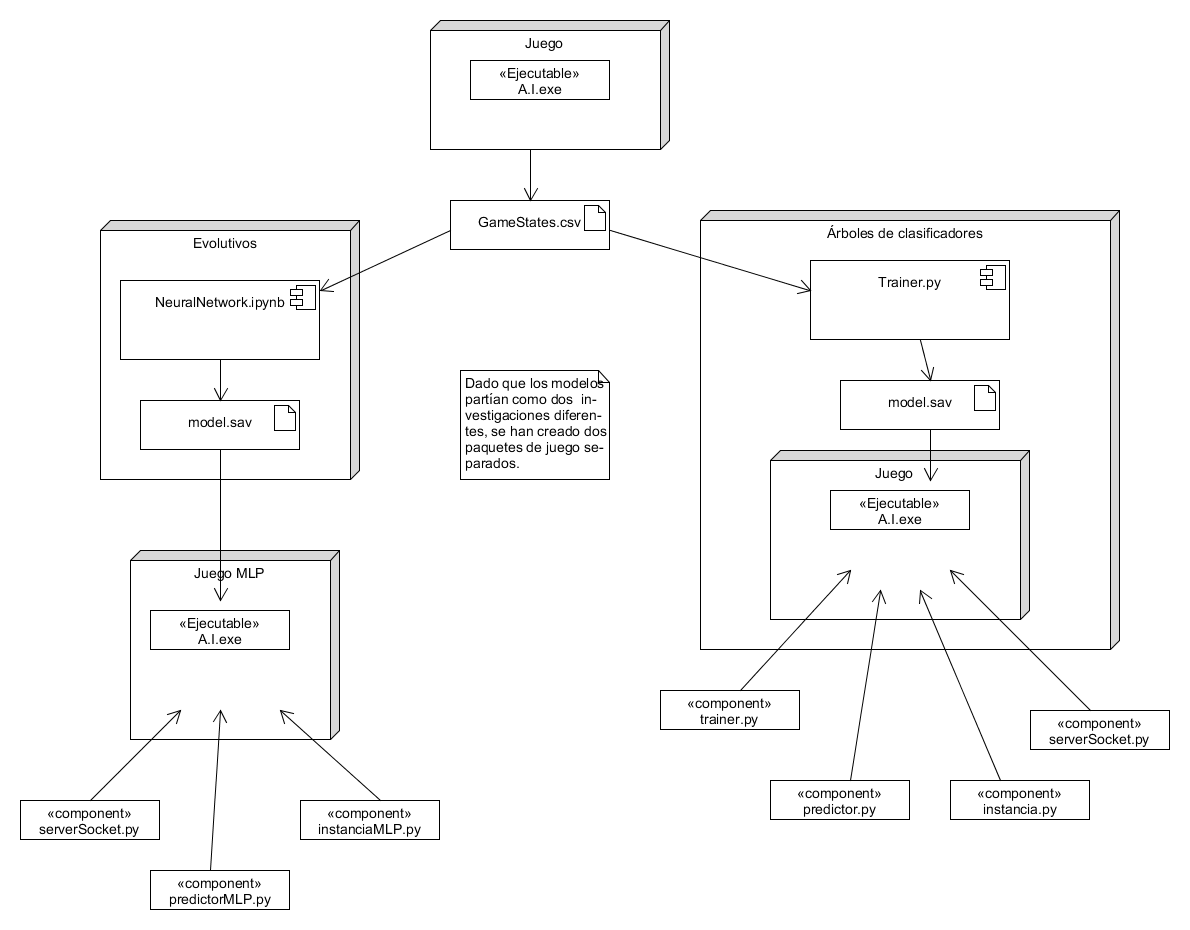
\includegraphics[width=\textwidth]{despliegue}
    \caption{Diagrama de despliegue}
    \label{fig:d_desp}
\end{figure}


\subsection {Diagrama de secuencias}
En esta sección se pretende aclarar el funcionamiento de, al menos, uno de los agentes, ya que el otro es muy similar.

El entrenamiento y explotación del modelo de agente inteligente se realizan tres acciones. La captura de datos, para el entrenamiento por imitación, en entrenamiento utilizando el clasificador preferido y, para finalizar, la utilización del modelo entrenado sobre el juego. 


\begin{figure}
    \centering
    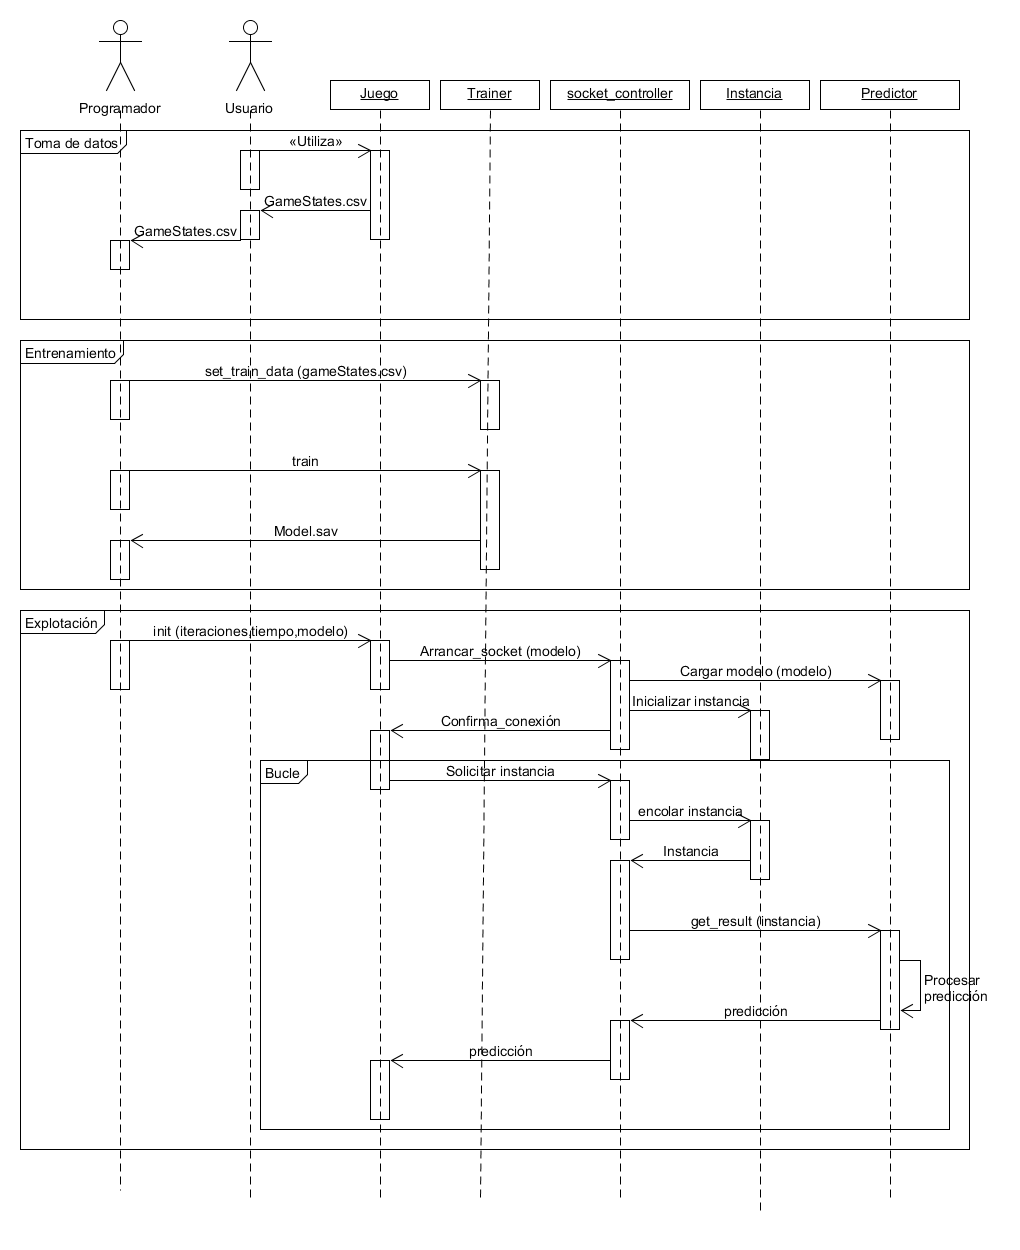
\includegraphics[width=\textwidth]{secuencias}
    \caption{Diagrama de secuencias (Arboles de decisión)}
    \label{fig:d_sec}
\end{figure}

\section{Diseño arquitectónico}

La captura de datos es muy sencilla: el jugador utiliza el juego normalmente y el juego crea un «log» con todas las instancias que se han ido generando a lo largo del juego. EL usuario deberá enviar al programador los resultados de la captura de datos de la partida para que este pueda trabajar con ellos.

El entrenamiento es muy sencillo y se compone de dos pasos. En primer lugar decimos al entrenador qué fichero de datos queremos utilizar. A continuación, una vez ha procesado todos los datos, se le indica que inicie el entrenamiento. Como resultado deberíamos obtener un modelo entrenado.

La explotación del modelo entrenado ya es algo más sofisticada, aunque sigue siendo un flujo relativamente sencillo.
\begin{itemize}
    \item 1 - El programador lanza el juego, indicando por parámetro el numero de rondas, el tiempo máximo por ronda y el modelo que tiene que utilizar.
    \item 2 - En cuanto se lanza el juego, este ejecuta un script de \emph{Python} que abre, a su vez, un socket con el que establecer la comunicación entre el juego y el agente inteligente.
    \item 3 - El script de \emph{Python}, además de abrir el socket, carga el modelo e inicializa el procesador de instancias.
    \item 4 - Realizados estos pasos el socket confirma la conexión y se comienzan a mandas las instancias de juego a este.
    \item 5 - Dado que el procesado de instancia se va a hacer en «paquetes» de cuatro, por el concatenado de instancias que se explica en la memoria, lo primero que hace el socket al recibir la instancia es encolarla.
    \item 6 - Una vez encolada, el procesador de instancias la devuelve junto con las tres anteriores.
    \item 7 - La instancia procesada se envía al «predictor» y éste, después de procesar internamente la predicción, la devuelve al servido de socket.
    \item 8 - EL servidor de socket devuelve la predicción al juego, que realizará la acción correspondiente.
\end{itemize}

Este proceso de envío, procesado y predicción se hace en bucle hasta que el jugador muera o se cierre el juego. El bucle se realiza cuatro veces por segundo.


\apendice{Documentación técnica de programación}

\section{Introducción}
En este apartado se detallará cómo entrenar nuestros agentes inteligentes y como hacerlos funcionar en el entorno del videojuego. 

\section{Estructura de directorios}

\section{Manual del programador}

\section{Compilación, instalación y ejecución del proyecto}

\section{Pruebas del sistema}

\apendice{Documentación de usuario}

\section{Introducción}

\section{Requisitos de usuarios}

\section{Instalación}

\section{Manual del usuario}







\bibliographystyle{plain}
\bibliography{bibliografiaAnexos}

\end{document}
